\chapter{Resultados y Conclusiones}

Para las pruebas realizadas se utilizo una computadora con un procesador AMD Phenom II 720 con tres núcleos a 2.80Ghz cada núcleo, 10 GB de memoria RAM y una tarjeta gráfica NVIDIA GeForce GTX 650 Ti tiene una arquitectura Kepler con 768 núcleos CUDA, memoria de 2 GB y un ancho de banda para 86.4 GB/s. En cuanto al software las pruebas de hicieron bajo un sistema operativo xubuntu 14.04, utilizando opencv y CUDA 6.5.

\section{Resultados}

Hay dos imágenes que fueron las que me ayudaron a realizar paso a paso este desarrollo, la primera es la de la Figura 5-1 es un castor y la 
segunda es la de la Figura 5-2 de un gato. La razón de por la cual tome estas dos imágenes fue, por que la del castor es una imagen pequeña y la de el gato es bastante grande, a su vez el castor cuenta con pocos puntos característicos contrario al gato que en todas las pruebas que realice fue el que mas puntos característicos tiene. Lo que quiero dar a entender es que tome los extremos en cuanto a los datos de entrada. 

\begin{figure}[ph]
			\centering
				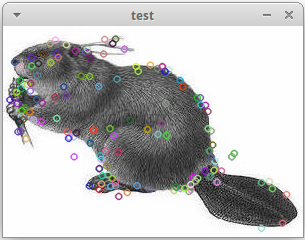
\includegraphics[scale=1]{img/castor.png}
			\caption{Puntos característicos encontrados en la imagen del castor}
\end{figure}


\begin{figure}[ph]
			\centering
				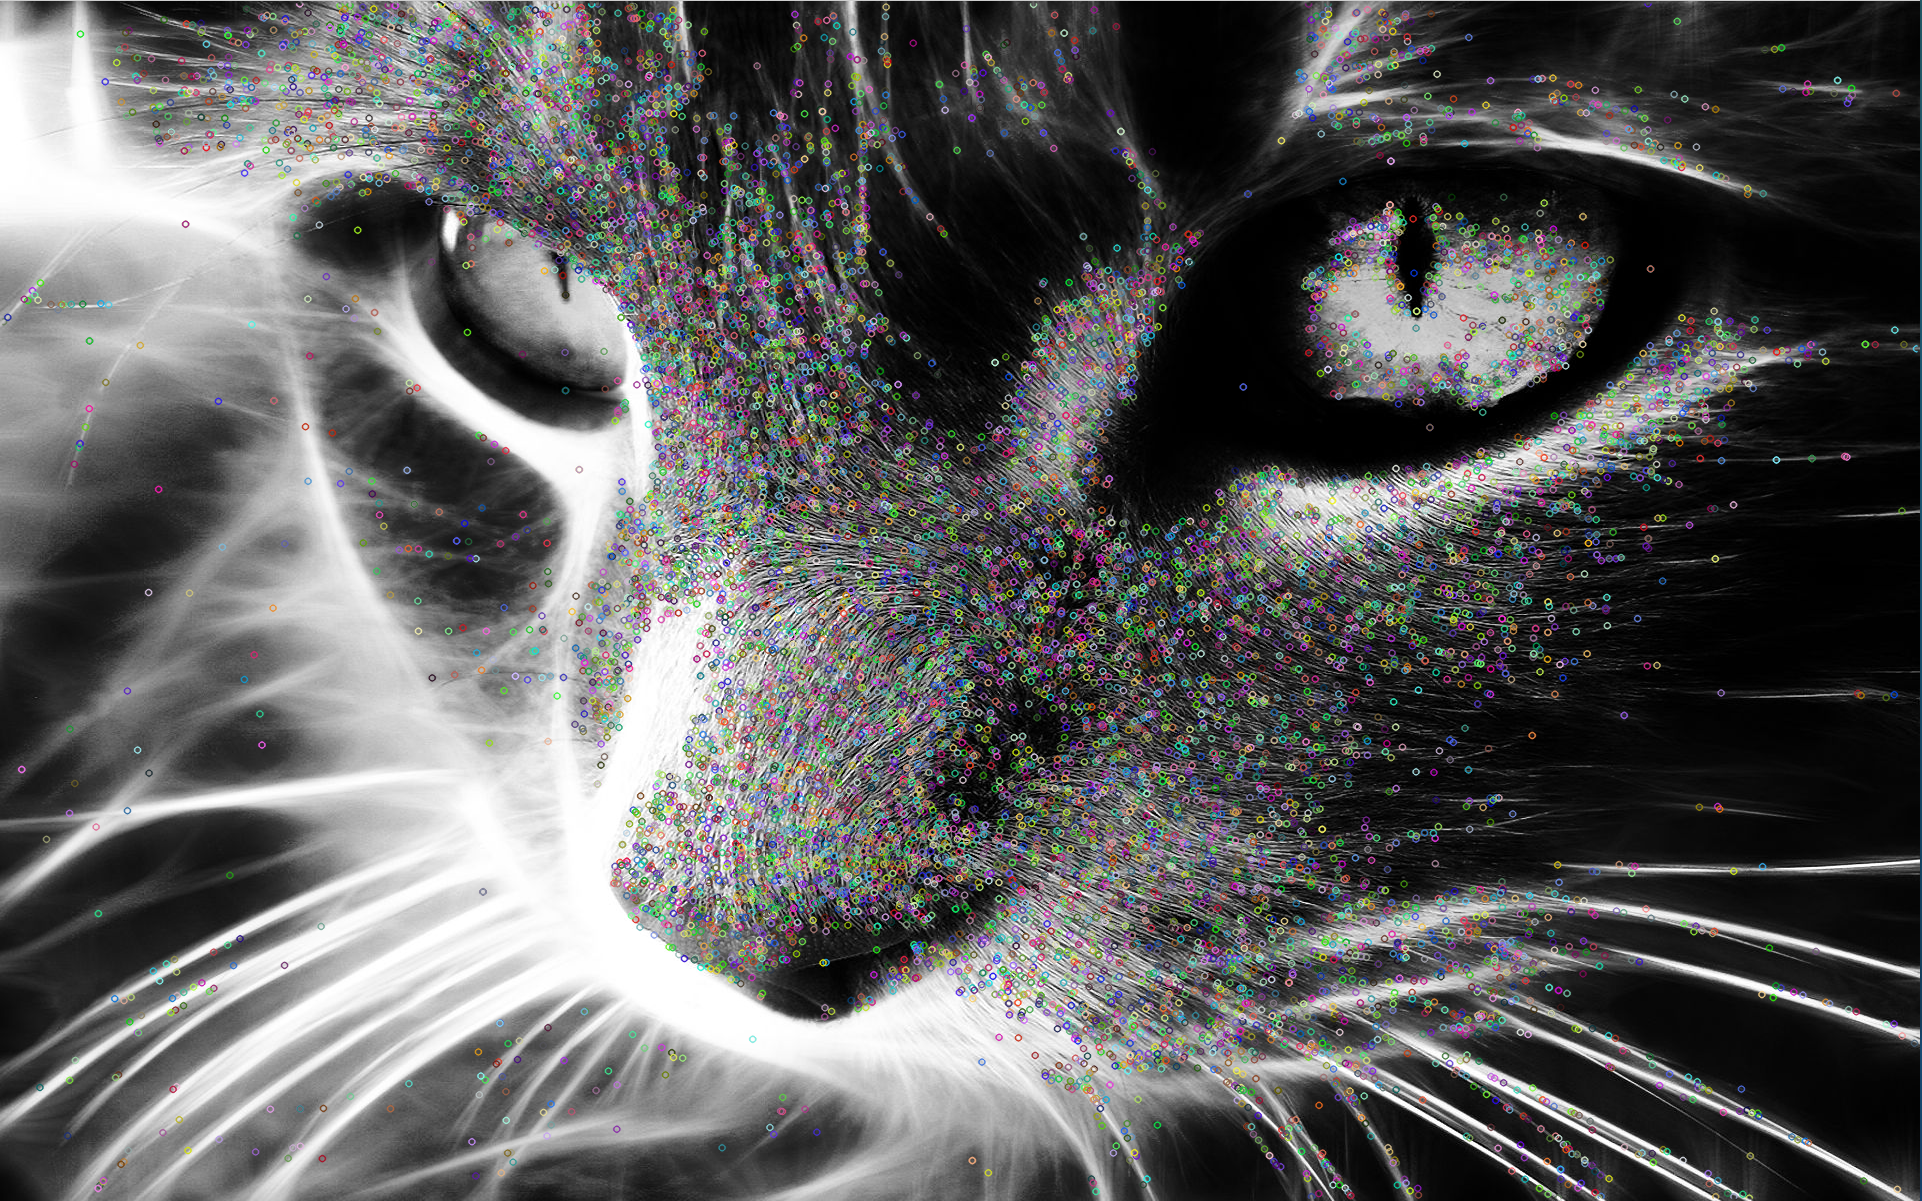
\includegraphics[scale=0.25]{img/gato.png}
			\caption{Puntos característicos encontrados en la imagen del gato}
\end{figure}


La primer prueba que hice con el castor y el gato, consistieron en medir el tiempo que tardaban en ejecutarse ciertas secciones del código de una implementación abierta de SIFT llamada Open SIFT, la cual se usa para la detección de objetos en el robot Justina, y en la implementacion de SIFT con CUDA que realice para obtener los puntos característicos. Podemos observar en las tablas 5-1 y 5-2 los resultados de estas pruebas. Las unidades de el tiempo es en milisegundos.
\pagebreak


\begin{table}[phtb]
\centering
\begin{tabular}{|l|c|c|}
\hline

\multicolumn{3}{|c|}{Castor} \\
\cline{1-3}
Partes de SIFT & CUDA SIFT & Open SIFT\\
\hline \hline
 Espacio escala DoG      & 17.25   &  29.32                        \\ \cline{1-3}
 Detección de PC         & 1.87    &  \multirow{2}{1cm} {50.09}    \\ \cline{1-2}
 Eliminación de PC malos & 0.75    &                               \\ \cline{1-3}
 Orientación de PC       & 8.80    &  12.35                        \\ \cline{1-3}

\end{tabular}
\caption{La resolución de la imagen es de 300x211 px y se encontraron 120 puntos característicos}
\label{tabla:final}
\end{table}


\begin{table}[phtb]
\centering
\begin{tabular}{|l|c|c|}
\hline

\multicolumn{3}{|c|}{Gato} \\
\cline{1-3}
Partes de SIFT & CUDA SIFT & Open SIFT\\
\hline \hline
 Espacio escala DoG      & 473.33  &  957.19                       \\ \cline{1-3}
 Detección de PC         & 55.47   &  \multirow{2}{1cm} {2210.82}  \\ \cline{1-2}
 Eliminación de PC malos & 9.82    &                               \\ \cline{1-3}
 Orientación de PC       & 125.2   &  1014.89                      \\ \cline{1-3}

\end{tabular}
\caption{La resolución de la imagen es de 1920x1200 px y se encontraron 12000 puntos característicos}
\label{tabla:final}
\end{table}

%





L que podemos notar de estos resultados de las tablas 5-1 y 5-2 es la aceleración al crear el espacio escala de DoG es de 1.85 veces mas rápido en el GPU, en las secciones de detección y eliminación de Puntos Característicos(PC) tenemos la mayor aceleración, siendo de hasta 40.66 veces mas, las anteriores aceleraciones son promedio entre la de la imagen del gato y el castor por que no eran cifras tan lejanas, pero en la parte de la orientación podemos notar como con imágenes mas grandes es más rápido procesarlas en el GPU, teniendo una aceleración de 8.10 veces para el gato y solo una aceleración de 1.40 para el castor.\\
Lo que hice después, fue medir el tiempo en que se tardaban en obtener los puntos característicos 3 diferentes implementaciones, la primera la que desarrolle para CUDA, la de OpenSIFT y por ultimo la que se encuentra en OpenCV. Podemos ver los resultados obtenidos en la tabla 5-3. 





\begin{table}[htb]
\centering
\begin{tabular}{|c|c|c|c|c|}
\hline

\multicolumn{5}{|c|}{Castor} \\
\cline{1-5}
Resolución & CUDA SIFT & Open SIFT & Opencv SIFT & Puntos Característicos\\
\hline \hline
 320 x 240  & 31.87   &   93.22  &  49.42   & 120\\ \cline{1-5}
\hline \hline
\multicolumn{5}{|c|}{Gato} \\
\cline{1-5}
Resolución & CUDA SIFT & Open SIFT & Opencv SIFT & Puntos Característicos\\
\hline \hline
1920x1200  & 676.32 &  4221.41 & 1415.98   & 12000\\ \cline{1-5}


\end{tabular}
\caption{Las unidades de tiempo son en milisegundos y la resolución en pixeles}
\label{tabla:final}
\end{table}






\pagebreak


Pero estas imágenes no eran las más adecuadas para hacer pruebas, ya que el robot de servicio Justina trabaja con imágenes como las de las figuras 5-3, 5-4, 5-5 y 5-6. Las primeras tres son objetos que tiene que manipular, la figura 5-6 es donde tiene que localizar los objetos.
Lo que hice fue medir cuanto tiempo se tardaban en generar los puntos característicos las 3 implementaciones anteriormente mencionadas y cambiar las resoluciones de estas imágenes. Los resultados los podemos ver a continuación en las siguientes tablas:


\begin{figure}[ph]
			\centering
				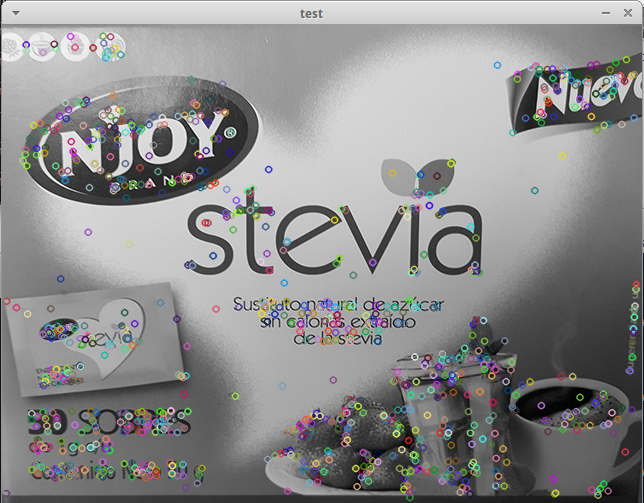
\includegraphics[scale=0.70]{img/stevia.png}
			\caption{Puntos característicos encontrados en la imagen del stevia}
\end{figure}


\begin{table}[phtb]
\centering
\begin{tabular}{|c|c|c|c|c|}
\hline

\multicolumn{5}{|c|}{Stevia} \\
\cline{1-5}
Resolución & CUDA SIFT & Open SIFT & Opencv SIFT & Puntos Característicos\\
\hline \hline
 320 x 240  & 31.87   &   151.10  &  49.42   & 370\\ \cline{1-5}
 640 x 480  & 97.91   &   484.64  &  182.46  & 920\\ \cline{1-5}
1280 x 960  & 335.05  &  1751.10  &  679.60  & 2800\\ \cline{1-5}
2560 x 1920 & 1251.38 &  5911.26  &  2893.68 & 3000\\ \cline{1-5}

\end{tabular}
\caption{Las unidades de tiempo son en milisegundos y la resolución en pixeles}
\label{tabla:final}
\end{table}


\begin{figure}[ph]
			\centering
				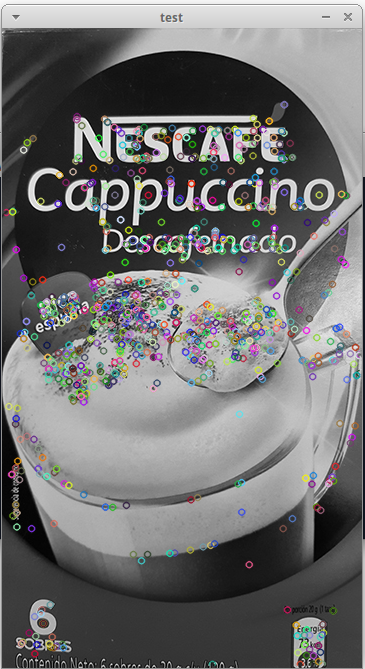
\includegraphics[scale=0.75]{img/cafe.png}
			\caption{Puntos característicos encontrados en la imagen del café}
\end{figure}

\begin{table}[phtb]
\centering
\begin{tabular}{|c|c|c|c|c|}
\hline

\multicolumn{5}{|c|}{Café} \\
\cline{1-5}
Resolución & CUDA SIFT & Open SIFT & Opencv SIFT & Puntos Característicos\\
\hline \hline
 320 x 180  & 30.25  &  117.95  & 39.25   & 290\\ \cline{1-5}
 640 x 360  & 81.91  &  484.64  & 182.46  & 760\\ \cline{1-5}
1280 x 720  & 284.57 &  1415.27 & 518.27  & 2800\\ \cline{1-5}
2560 x 1440 & 993.96 &  4963.27 & 1951.21 & 7000\\ \cline{1-5}

\end{tabular}
\caption{Las unidades de tiempo son en milisegundos y la resolución en pixeles}
\label{tabla:final}
\end{table}

\begin{figure}[ph]
			\centering
				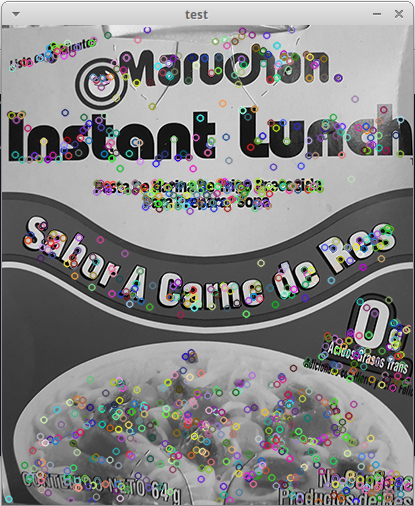
\includegraphics[scale=1]{img/sopa.png}
			\caption{Puntos característicos encontrados en la imagen de la sopa}
\end{figure}

\begin{table}[phtb]
\centering
\begin{tabular}{|c|c|c|c|c|}
\hline

\multicolumn{5}{|c|}{Sopa} \\
\cline{1-5}
Resolución & CUDA SIFT & Open SIFT & Opencv SIFT & Puntos Característicos\\
\hline \hline
 206 x 240  & 28.10  &  130.98  & 37.78   & 425\\ \cline{1-5}
 411 x 480  & 74.43  &  412.04  & 129.49  & 1000\\ \cline{1-5}
 802 x 906  & 241.83 &  1400.59 & 469.07  & 3000\\ \cline{1-5}
1645 x 1920 & 850.29 &  4478.54 & 1674.67 & 3900\\ \cline{1-5}

\end{tabular}
\caption{Las unidades de tiempo son en milisegundos y la resolución en pixeles}
\label{tabla:final}
\end{table}




\begin{figure}[ph]
			\centering
				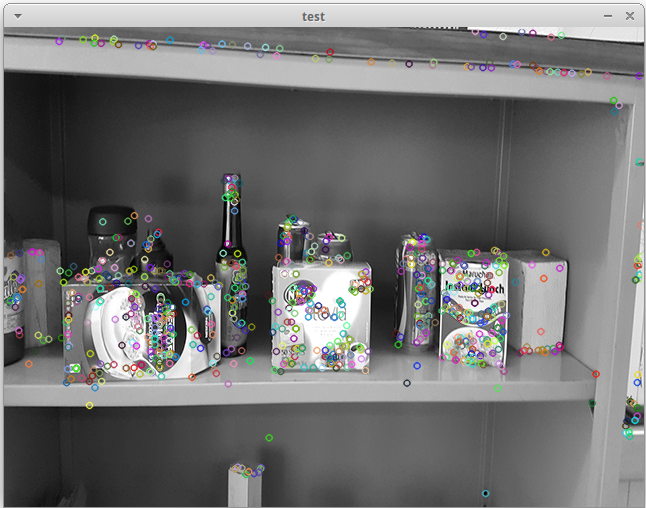
\includegraphics[scale=0.75]{img/estante.png}
			\caption{Puntos característicos encontrados en la imagen del estante}
\end{figure}


\begin{table}[phtb]
\centering
\begin{tabular}{|c|c|c|c|c|}
\hline

\multicolumn{5}{|c|}{Estante} \\
\cline{1-5}
Resolución & CUDA SIFT & Open SIFT & Opencv SIFT & Puntos Característicos\\
\hline \hline
 320 x 240  & 33.45   & 130.24   & 47.52   & 210\\ \cline{1-5}
 640 x 480  & 101.20  &  451.39  & 177.28  & 700\\ \cline{1-5}
1280 x 960  & 340.92  &  1602.51 & 669.09  & 2100\\ \cline{1-5}
2560 x 1920 & 1275.37 &  6031.39 & 3037.60 & 3700\\ \cline{1-5}

\end{tabular}
\caption{Las unidades de tiempo son en milisegundos y la resolución en pixeles}
\label{tabla:final}
\end{table}

Un factor que creí afectaría el tiempo de ejecución de todos los programas fue la cantidad de puntos característicos que existen en la imagen, cosa que no paso, podemos observar como se repite el fenómeno que notamos con el castor y el gato. Entre mas grande es la imagen obtenemos una aceleración mas grande esto paso para todos los casos en las imágenes anteriores. Me parece importante mencionar que el tiempo medido en las tablas incluye el cuello de botella que existe al estar pasando datos de la memoria RAM de la computadora a la memoria de la GPU.     

\pagebreak
\section{Conclusiones}

 Las pruebas a las que es sometido el robot de servicio Justina, cada vez son más rigurosas,los sistemas deben ser cada vez más rápidos y confiables. También las nuevas generaciones de sensores son mucho mejores tenemos mas información para analizar, actualmente se utiliza un sensor Kinect para obtener las imágenes, esta tiene una resolución de  640 x 480 px y se utiliza el código de openSIFT para procesar esta imágenes, después     se adquirió una cámara RGB logitech C920 que tiene una  de 1920 x 1080 px, el procesamiento de la imagen fue mucho mas lento. Se planea empezar a usar también el nuevo sensor de Microsoft Kinect 2 el cual también tiene una resolución de 1920 x 1080 px. 
 
 
 Los resultados obtenidos tiene dos matices a mi parecer, donde las imágenes son muy pequeñas y hay poco que procesar , cuando el robot necesita encontrar objetos en una mesa, segmenta los objetos de la mesa y quedan solo los objetos, que no tienen una cantidad muy grande de pixeles a procesar, por lo que aun que es un poco más rápido procesarlos en el GPU, no tiene gran aceleración en comparación a la librería de OpenCV y es mucho mas sencillo implementarlo; la otra parte es que se ha estado trabajando para que Justina no solo encuentre objetos en la mesa sino que debe tener capacidad para encontrarlos en un libreo o estante. En el laboratorio de BioRobotica de la UNAM  se ha estado tratando de segementar estos estantes o libreros para poder seguir con la misma metodología al momento de buscar objetos, cosa que no se a logrado con éxito total. Lo que se implemento fue hacer una búsqueda de los objetos en toda la imagen, para esto se intento hacer con las imágenes que entrega el Kinect, pero la baja calidad de la imagen no permitía encontrar los objetos, ya que la distancia de donde se tomaba la foto era mas lejos de lo que acostumbra ser.
 Se cambio la fuente de la imagen por la cámara C920 y los resultados mejoraron, pero el tiempo de procesamiento aumento.

EL robot Justina participa en una competencia principalmente llamada Robocup, en 2015 se puso una nueva prueba llamada  \textit{Manipulation and object recognition} donde se tenia que buscar objetos en un librero y manipularlos básicamente. Para esta prueba solo dan 3 minutos para reconocer y manipular objetos,  de los cuales nosotros gastamos todo el tiempo solo reconociendo, ya que con una sola foto no podríamos analizar todos los objetos que  hay en el librero, por lo cual hay que hacer varias tomas de diferente ángulos.


 
 A lo que me quiero referir es que la cantidad de datos que se tienen que procesar crecieron solo tres veces y se tarda en procesar hasta 13 veces mas tiempo que con las anteriores resoluciones, lo que a mi parecer es una buena idea voltear a ver a las tarjetas gráficas de propósito general, las cuales ya se cuentan con ellas en las laptops que el robot usa. Observando los resultados con resoluciones de 1920 x 1080 podemos ver una aceleración de hasta 5 veces respecto a OpenSIFT y 2 veces contra la librería OpenCV, ya que en lugar de que el proceso tarde 5 segundos por foto estaría tardando solo un segundo.  
 
  





 
 
 
 
 
 
 
 
 

